% Thesis template by Aleksander M. Stensby
% aleksander.stensby@gmail.com

%\documentclass[12pt,letterpaper,final]{report}
\documentclass[12pt,a4paper,final]{report}
\usepackage[utf8]{inputenc}
\usepackage{makeidx}
\usepackage{varioref}
\usepackage{setspace}
\usepackage{times}    % Use this package for times-font.
\usepackage{fancyvrb}
\usepackage{moreverb}
\usepackage{fancyhdr}
\usepackage{epsfig}
\usepackage{eucal}
\usepackage{amsmath}
\usepackage{amsfonts}
\usepackage{floatflt}
\usepackage{tocbibind}
\usepackage{wrapfig}
\usepackage{listings}
\usepackage{color}
\usepackage{amsthm}
\usepackage{subfigure}
\usepackage{longtable}
\usepackage{url}
\usepackage{multicol}
\usepackage{array}
\usepackage[style=list,toc=true]{glossaries}
\usepackage{graphicx}     % For inclusion of images
\usepackage{uiafrontpage} % For UiA Style frontpage.
\usepackage{rotating}
\usepackage{gnuplottex}

\definecolor{Brown}{cmyk}{0,0.81,1,0.60}
\definecolor{OliveGreen}{cmyk}{0.64,0,0.95,0.40}
\definecolor{Keyword}{cmyk}{0.66,0.90,0.33,0.20}
\definecolor{Comment}{cmyk}{0.88,0.35,1.00,0.30}
\definecolor{Identifier}{cmyk}{1,1,1,1}
\definecolor{XmlKeyword}{cmyk}{0.66,0.90,0.33,0.20}
\definecolor{FrameColor}{cmyk}{0.66,0.90,0.33,0.20}
\definecolor{XmlIdentifier}{cmyk}{0,0.81,1,0.60}
\definecolor{XmlString}{cmyk}{1,1,1,1}


%%%% Fancy
% 11pt font
%\headheight=13.6 pt

% 12pt font
\headheight=14.5 pt

\pagestyle{fancy} 
\fancyhead[L]{\leftmark}
\fancyhead[R]{}
%lowercase
%\renewcommand{\chaptermark}[1]{\markboth{#1}{}}

%Fit more figures on a page
\renewcommand{\topfraction}{.99}
\renewcommand{\bottomfraction}{.99}
\renewcommand{\textfraction}{.01}
\renewcommand{\floatpagefraction}{.99}

% spacing:
%\singlespacing
\onehalfspacing
%\doublespacing

\theoremstyle{definition}
\newtheorem{theorem}{Theorem}
\hyphenation{theorem}
\newtheorem{definition}{Definition}
\newtheorem{remark}{Remark}

\oddsidemargin=0.5in \evensidemargin=0.3in
\parskip=0.0 true in

\author{Bjørnar Hansen, Håkon Bakkevig Steinsholt and Daniel Aasen}
\titlelogo{images/uia_logo_large} % Path to UiA logo.
\title{Gaussian Processes for Analysis of Thompson Sampling Based Solutions to 
the Goore Game }
\reporttype{Advanced Project}

\draftversion{0.1}
\date{\today} % Specify own date

\makeglossaries

% For draft work, select the chapters to include in the pdf but still keep all 
% cross-references intact.
% \includeonly{background}

\begin{document}

    \maketitle

    \newpage    
    \begin{abstract}

The use of learning automata employing the Thompson sampling method for solving 
the stochastic multi-armed bandit problem is well known, but confusion surrounds 
the all-important parameter for this algoritm -- the observation noise. In this 
paper we investigate how this parameter affects the outcome of bandit 
simulations. We also test this in a Goore game setting where the players are 
modelled as learning automata playing 2-armed bandits.

\end{abstract}

    \chapter*{Preface}
(What and why)
This report is going into how Goore game and Multi armed bandits work,
and aims to improve the knowledge on how to determine the values of the 
variables that the creator needs to set. Reason for this is to help improve
usage of these problems and research.

(Limitations ect.)
We are only investigating Thompson sampling in this report. We are not going 
over 10 000 rounds and 100 000 iterations for the test we have done. Also the
range of the opservasion noice we have used is from approximately 0 to 5.

(Write what you can conclude in this report)

    \tableofcontents
    \listoffigures
    \listoftables

    \parskip=0.1 true in

    \newpage

    % General structure, normally (background, and solution chapter may be split 
    % into several different chapters!
    \chapter{Introduction}
\label{ch:introduction}

\textit{Approx. 10 pages}

This document forms a general structure for a thesis.
Normally, background, and solution chapter may be split into several different chapters!

\section{Introduction}
In this report we investigated what might be are the best observation noise for different 
types of bandits and Goore games. By changing the bandits with adding more arms or changing the values 
of the arms, then recorded the simulations to see what difference it made to the simulation. Then check 
what are the best possible observation noise are in that case.
\section{Motivation}

\section{Goal}
Goal of the thesis.

\subsection{Field of research}

\section{Thesis definition/objective / Statement of the Problem}

\section{Contributions}
 
\section{Target audience}


\section{Report outline / Thesis Organization}
    
    \chapter{Background}
\label{ch:background}

\section{Reinforcement learning}
\begin{figure}[htbp]
    \centering
    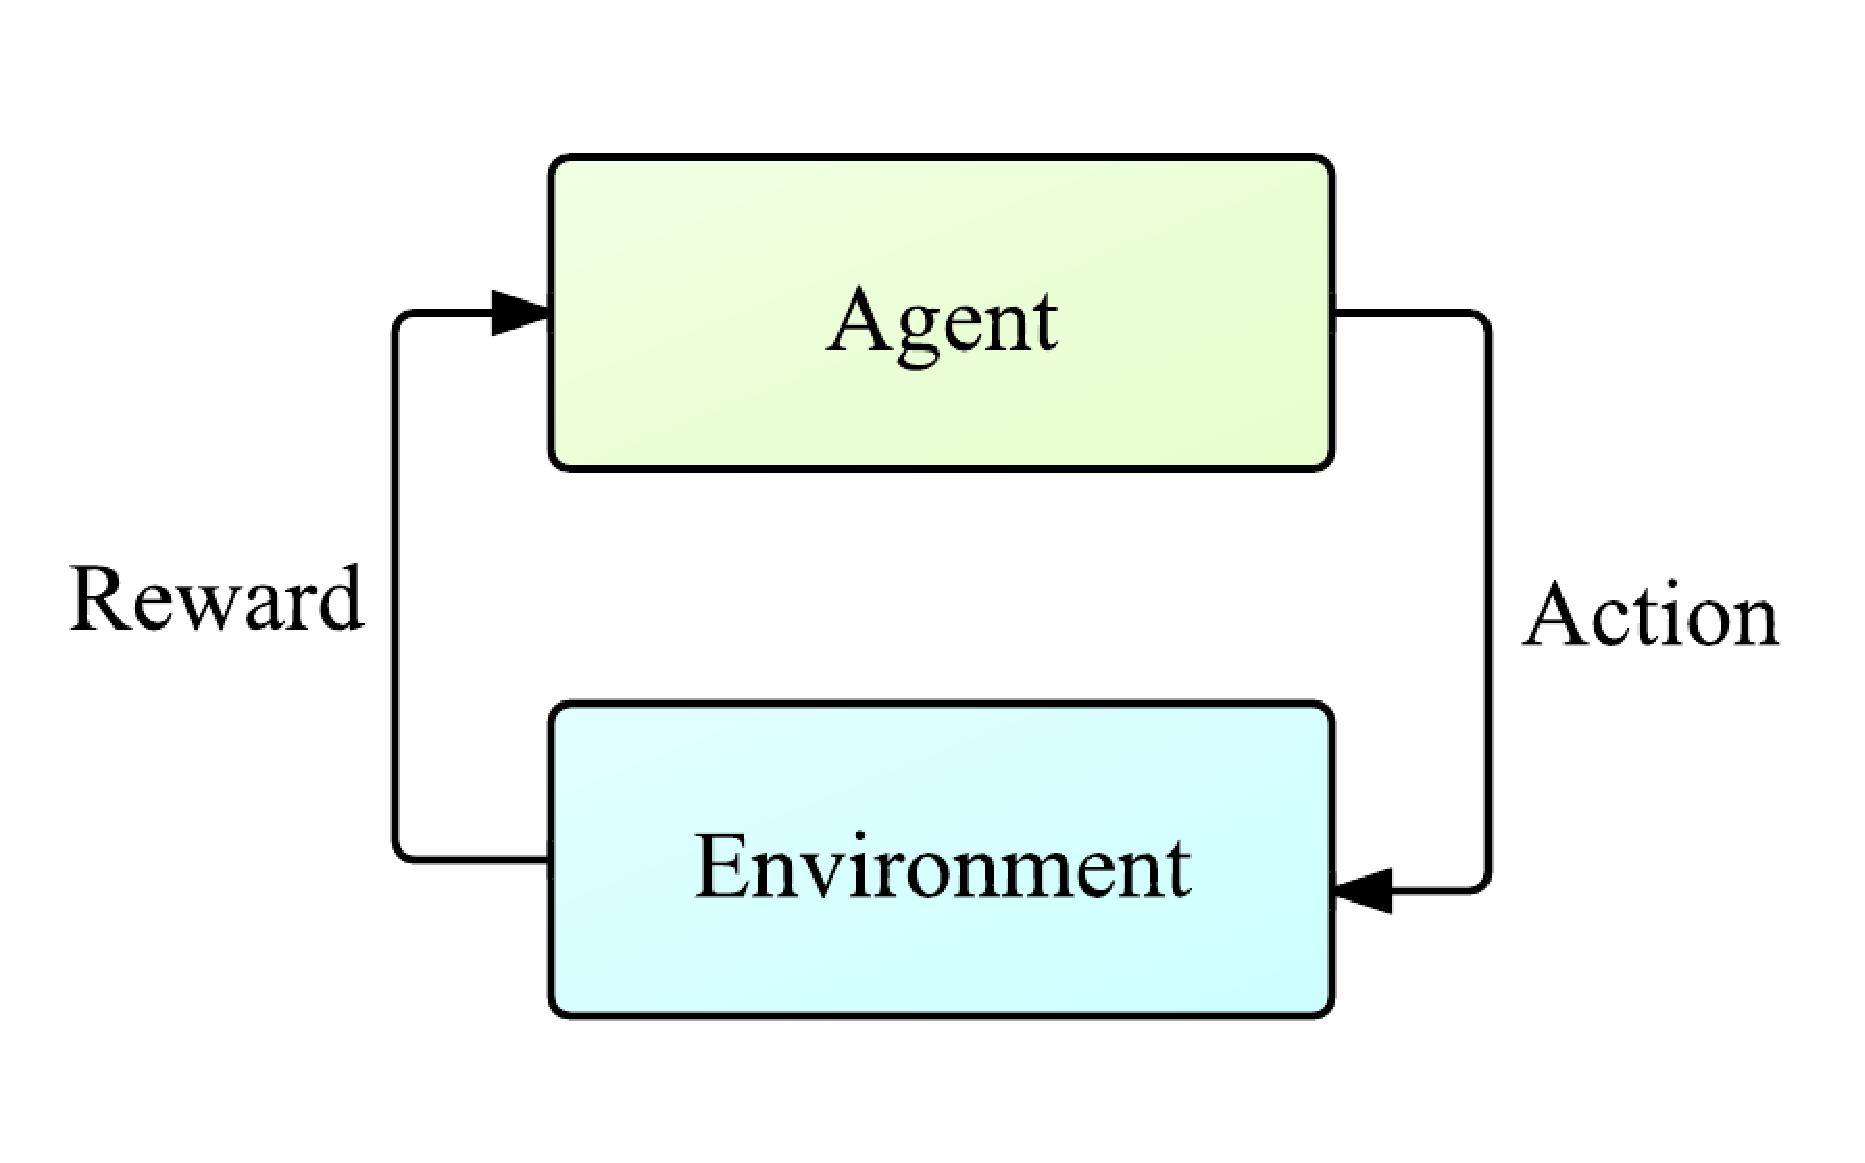
\includegraphics[width=8cm]{images/ReinforcementLearning}
    \label{fig:rlearn}
    \caption{Simplified reinforcement learning model}
\end{figure}

In our simplified model of reinforcement learning, illustrated in figure~\ref{fig:rlearn}, one can observe the basic flow of actions. On every iteration the agent takes an action and receives a reward from the environment based on that action.
This feedback is then used by the agent to learn about the environment.
By repeatedly choosing actions and receiving feedback from the environment, the agent is able to decide which action is the most profitable.
The more general version of reinforcement learning includes a communication of the environment's state to the agent, but in our case the environment does not change state and therefore this particularity is omitted from the figure.
A comprehensive survey of reinforcement learning is found in \cite{Kaelbling1996}.

The goal of the agent is to maximise the rewards received in the long term.
This performance measure can equivalently be defined as minimising \emph{regret}, that is, minimising the difference between actual received rewards and the rewards that arise from always choosing the optimal action.
We talk of two types of regret:
Total regret $R_T$, where we consider the total sum of rewards, and instantaneous regret $R_I(t)$, where we consider the reward received at a specific point in time.
\begin{align*}
    R_I(t) &= \mu^* - r_t \\
    R_T &= T\mu^* - \sum_{t=1}^{T}{r_t} = \sum_{t = 1}^{T}{R_I(t)} 
\end{align*}

Given that the environment normally is considered to be stochastic, the agent has to weigh exploration against exploration.
Actions have variable rewards associated with them, and exploration is needed to estimate the real expected payoff of each action, but if the agent allocates too much or too little time for exploration, its total reward suffers.
Thus the agent has to decide on whether to continue exploration -- to get a clearer picture of which action is the optimal one -- or to exploit the knowledge it already has acquired and select the action it currently believes to be the best one.

\section{The multi-armed bandit problem}
The simplest \cite{Kaelbling1996} way to model reinforcement learning problems is through the multi-armed bandit scenario.
Imagine the iconic gambling machine found in any self-respecting casino, only this version of the apparatus has more than one arm with which a player may try her luck.
The arms may cause the machine to give the player different rewards, so she will want to choose the arm which gives the highest payoff.
Hence, a strategy for optimising the machine's payout must be employed.

Before any arm-pulling has been done, nothing is known about the possible payoffs from the available arms except that some arms are better than others -- obviously our player will profit the most from playing only the best arm.
And now we again see the dilemma of exploration and exploitation: she must make a trade-off between exploration 
-- discovering which arm is truly the best one -- and exploitation -- actually picking the best arm.
When selecting to explore the short-term reward is sacrificed for possible long-term payoffs, while exploitation may cause the player to not achieve the best reward possible due to incomplete knowledge of the search space.

In this paper we look at Gaussian bandits, as opposed to the more common Bernoulli bandits.
This entails that arms are normally distributed, and each arm is described simply by a mean and variance.
The choice of Gaussian distributions is also due to the fact that the Thompson sampling algorithm requires distributions with conjugate priors -- the normal distribution is self-conjugate.


\section{The Goore Game}
Introduced by Tsetlin \cite{Tsetlin1964} in 1964, the Goore game\footnote{Also known as the Gur game.} is an iterated cooperation game where each player is not privy to information on the other players.
It can be described as a voting process where the referee knows the correct answer, and the players cast their votes as simple ‘yes’ or ‘no’.
The correct answer is a certain fraction of yes-votes, and players are rewarded based on how close they collectively are to the ideal solution.
Rewards are determined by an unimodal performance criterion $G(\lambda)$, for instance the density of the normal distribution, where $\lambda$ is the fraction of yes-votes.
The fraction of yes-votes preferred by the referee corresponds to the maximum of the performance criterion; when the normal distribution is used it is simply the mean value of the distribution. 

The Goore game is inherently noisy, in that the reward for a single player is dependent on the actions of all the other players, resulting in reward variance.
The noise level is at its highest as $\lambda = 0.5$.
At this point the reward received by one player is severely dependent upon the other players choices, and so has the highest variance. 
Conversely, the lowest noise level is found when $\lambda = 0.0\text{ or } 1.0$, where on average the reward for a particular player always increases as any one player switch to the correct choice. 
In addition to the inherent noisiness of the game the feedback process itself may be noisy, typically modelled by adding Gaussian white noise to the rewards.

\begin{figure}[htbp]
\centering
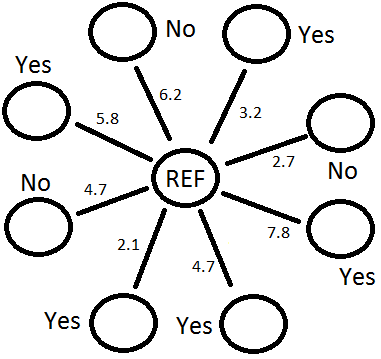
\includegraphics[height=70mm,width=70mm]{images/goore_game}
\caption{Eight Player Goore Game}
\label{fig:gg}
\end{figure}

At the start of the game all participants select an action at random, as seen in figure~\ref{fig:gg}.
The referee tallies the votes and based on the performance criterion it calculates the reward each player receive.
The players will then use the reward they received from the referee to decide on whether to change their vote or to stick with it the next round.
The differing rewards in figure~\ref{fig:gg} are due to noisy feedback from the referee: the players generally do not receive the same reward in a given round.
This is part of the uncertainty in the Goore Game, that a player can make a good choice and still receive a low
reward. 
Another factor that makes the game difficult is that only the referee knows the performance criterion.
The players simply vote and receive a reward as feedback.

As the performance criterion is unimodal there is a unique fraction of yes-votes that yields the maximum reward.
For the remainder of this paper the performance criterion will be, as suggested earlier, the density of a Gaussian distribution, an example of which is given in figure~\ref{fig:gfunc}.
In the figure $\lambda$ is the fraction of players that vote yes and $\lambda^*$ is the target value, here 0.5, for which the referee provides the highest expected reward.
If the players reach the target value they are not ensured a high reward, due to the noisy environment, but the players all receive the highest possible expected reward by staying in this configuration.

\begin{figure}[htbp]
\centering
\begin{gnuplot}[terminal=epslatex,terminaloptions=color solid]
set style data lines
set nokey
set xlabel '$\lambda$'
set ylabel '$G(\lambda)$'
set xrange[-0.25:1.25]
#set yrange[0:2]
set label '$\lambda^*$' at 0.55, 0.6
set arrow from 0.5,2 to 0.5,0 nohead lt 0 lw 3
plot (1/(0.2*sqrt(2*pi))) * exp((-0.5)*(((x-0.5)/0.2)**2)) lw 3
\end{gnuplot}
\caption{An unimodal performance criterion}
\label{fig:gfunc}
\end{figure}

\section{Local Thompson sampling}
Local Thompson sampling (LTS) \cite{May2011} is based on a sampling technique pioneered by Thompson \cite{Thompson1933} in 1933. 
The method is Bayesian in nature, in that it uses new information to update probability estimates, but avoids the computational intractability that is often the drawback of Bayesian methods.
While the original method Thompson proposed was for choosing between 2 actions in a Bernoulli trial, it is easily generalised as a method of choosing among any number of actions with arbitrary reward distributions.
The \emph{local} part of the name is unimportant in our setting as the mean reward values are fixed, but it relates the fact that actions selection is done taking into account the current regressor (which is a value determining the mean reward for each action).

The algorithm functions as follows: For every available action it keeps a distribution estimate.
On every round $t$, it picks an action by drawing a random number from each distribution and selecting the action which achieved the highest value.
Using the reward $r_i$ which is then received, the arm estimate of the selected arm $i$ is updated.
Specifically, in the Gaussian bandit setting the mean and variance is calculated as follows \cite{Murphy2007}:
\begin{align*}
    \mu_i [t + 1] &= \frac{\sigma_i^2 [t] \cdot r_i + \sigma_{ob}^2 \cdot \mu_i [t]}{\sigma_i^2 [t] + \sigma_{ob}^2} \\
    \sigma_i^2 [t + 1] &= \frac{\sigma_i^2 [t] \sigma_{ob}^2}{\sigma_i^2 [t] + \sigma_{ob}^2} = \left(\frac{1}{\sigma_{ob}^2} + \frac{1}{\sigma_i^2 [t]} \right)^{-1} \text{,}
\end{align*}
where $\sigma_i^2 [t + 1]$ and $\mu_i [t + 1]$ is, respectively, the variance and mean of the updated arm.
The term $\sigma_{ob}$, the observation noise, is the parameter which is investigated in this report.
It is assigned a value akin to a learning rate: A low value signifies that new information should be given much importance, while a high value means that new observations are lightly weighted.
At the same time the \ob{} can be thought of as a discount factor, as it determines the rate of exploration versus exploitation.
This is illustrated in figure~\ref{fig:variance}. 
It shows how the variance of the estimates develops as a function of $t$, for the cases where $\sigma_{ob}^2 \in \{0.0001, 1.0\}$, with $\sigma_i [0] = 50$ for all $i$.
We see that the observation noise value determines how fast the variance shrinks and what it converges towards, and hence, how much time to allocate for exploration.

\begin{figure}[htbp]
    \centering
%% Haskell code to generate data %%
% let var v ob = let vv = (v*ob)/(v+ob) in vv : var vv ob
% let ppB b = unlines $ map ppL b
% let ppL (t,a,b,c) = show t ++ " " ++ show a ++ " " ++ show b ++ " " ++ show c
% writeFile "est.txt" . unlines . map ppB . transpose 
%   $ map (\(est, ob) -> (zip4 (var est ob) ([1..10000]) (repeat est) (repeat ob)))
%         [(est, ob) | est <- [2500],
%                      ob <- ([0.001,0.002, 0.003, 0.006, 0.01, 0.03,0.06] ++ [0.1,0.2..3.0])]
%
%% 3D plot %%
%    \begin{gnuplot}[terminal=epslatex,terminaloptions=color solid]
%    set grid
%    set ylabel "[r]{\\shortstack{Observation noise \\\\ ($\\sigma_{ob}^2$)}}" offset 6,-2
%    set xlabel 'Rounds' offset 0,-0.5
%    set zlabel 'Variance estimate ($\hat{\sigma}^2$)' rotate offset -0.5,0
%    set xyplane 0
%    set log z; set log cb
%    set xrange [0:1000]
%    set zrange [1e-06:3]
%    set ytics 0.4 offset 0,-0.5
%    set xtics offset 0,-0.5
%     set palette model CMY rgbformulae 7,5,15
%    splot 'est.txt' using 2:(column(4) < 1.5 ? column(4) : 1/0):(column(3) == 2500.0 ? column(1) : 1/0) every :::::1000 with pm3d title "" \
%    ,'est.txt' using 2:(column(4)<1.5?column(4):1/0):(column(3)==2500.0?column(1):1/0) every 2:100::50::1001 with line lt -1 lw 1 title "" \
%    ,'est.txt'       using 2:(column(4) < 1.5 ? column(4) : 1/0):(column(3) == 2500.0 ? column(1) : 1/0) every 2:10::::70  with line lt -1 lw 1 title ""
%    \end{gnuplot}
%    % GNUPLOT: LaTeX picture with Postscript
\begingroup
  \makeatletter
  \providecommand\color[2][]{%
    \GenericError{(gnuplot) \space\space\space\@spaces}{%
      Package color not loaded in conjunction with
      terminal option `colourtext'%
    }{See the gnuplot documentation for explanation.%
    }{Either use 'blacktext' in gnuplot or load the package
      color.sty in LaTeX.}%
    \renewcommand\color[2][]{}%
  }%
  \providecommand\includegraphics[2][]{%
    \GenericError{(gnuplot) \space\space\space\@spaces}{%
      Package graphicx or graphics not loaded%
    }{See the gnuplot documentation for explanation.%
    }{The gnuplot epslatex terminal needs graphicx.sty or graphics.sty.}%
    \renewcommand\includegraphics[2][]{}%
  }%
  \providecommand\rotatebox[2]{#2}%
  \@ifundefined{ifGPcolor}{%
    \newif\ifGPcolor
    \GPcolortrue
  }{}%
  \@ifundefined{ifGPblacktext}{%
    \newif\ifGPblacktext
    \GPblacktexttrue
  }{}%
  % define a \g@addto@macro without @ in the name:
  \let\gplgaddtomacro\g@addto@macro
  % define empty templates for all commands taking text:
  \gdef\gplbacktext{}%
  \gdef\gplfronttext{}%
  \makeatother
  \ifGPblacktext
    % no textcolor at all
    \def\colorrgb#1{}%
    \def\colorgray#1{}%
  \else
    % gray or color?
    \ifGPcolor
      \def\colorrgb#1{\color[rgb]{#1}}%
      \def\colorgray#1{\color[gray]{#1}}%
      \expandafter\def\csname LTw\endcsname{\color{white}}%
      \expandafter\def\csname LTb\endcsname{\color{black}}%
      \expandafter\def\csname LTa\endcsname{\color{black}}%
      \expandafter\def\csname LT0\endcsname{\color[rgb]{1,0,0}}%
      \expandafter\def\csname LT1\endcsname{\color[rgb]{0,1,0}}%
      \expandafter\def\csname LT2\endcsname{\color[rgb]{0,0,1}}%
      \expandafter\def\csname LT3\endcsname{\color[rgb]{1,0,1}}%
      \expandafter\def\csname LT4\endcsname{\color[rgb]{0,1,1}}%
      \expandafter\def\csname LT5\endcsname{\color[rgb]{1,1,0}}%
      \expandafter\def\csname LT6\endcsname{\color[rgb]{0,0,0}}%
      \expandafter\def\csname LT7\endcsname{\color[rgb]{1,0.3,0}}%
      \expandafter\def\csname LT8\endcsname{\color[rgb]{0.5,0.5,0.5}}%
    \else
      % gray
      \def\colorrgb#1{\color{black}}%
      \def\colorgray#1{\color[gray]{#1}}%
      \expandafter\def\csname LTw\endcsname{\color{white}}%
      \expandafter\def\csname LTb\endcsname{\color{black}}%
      \expandafter\def\csname LTa\endcsname{\color{black}}%
      \expandafter\def\csname LT0\endcsname{\color{black}}%
      \expandafter\def\csname LT1\endcsname{\color{black}}%
      \expandafter\def\csname LT2\endcsname{\color{black}}%
      \expandafter\def\csname LT3\endcsname{\color{black}}%
      \expandafter\def\csname LT4\endcsname{\color{black}}%
      \expandafter\def\csname LT5\endcsname{\color{black}}%
      \expandafter\def\csname LT6\endcsname{\color{black}}%
      \expandafter\def\csname LT7\endcsname{\color{black}}%
      \expandafter\def\csname LT8\endcsname{\color{black}}%
    \fi
  \fi
  \setlength{\unitlength}{0.0500bp}%
  \begin{picture}(7200.00,5040.00)%
    \gplgaddtomacro\gplbacktext{%
      \csname LTb\endcsname%
      \put(942,1180){\makebox(0,0){\strut{} 0}}%
      \csname LTb\endcsname%
      \put(1590,1061){\makebox(0,0){\strut{} 200}}%
      \csname LTb\endcsname%
      \put(2238,942){\makebox(0,0){\strut{} 400}}%
      \csname LTb\endcsname%
      \put(2886,824){\makebox(0,0){\strut{} 600}}%
      \csname LTb\endcsname%
      \put(3533,705){\makebox(0,0){\strut{} 800}}%
      \csname LTb\endcsname%
      \put(4180,586){\makebox(0,0){\strut{} 1000}}%
      \csname LTb\endcsname%
      \put(4398,646){\makebox(0,0){\strut{} 0}}%
      \csname LTb\endcsname%
      \put(4866,904){\makebox(0,0){\strut{} 0.4}}%
      \csname LTb\endcsname%
      \put(5333,1161){\makebox(0,0){\strut{} 0.8}}%
      \csname LTb\endcsname%
      \put(5801,1418){\makebox(0,0){\strut{} 1.2}}%
      \csname LTb\endcsname%
      \put(6268,1675){\makebox(0,0){\strut{} 1.6}}%
      \put(920,1384){\makebox(0,0)[r]{\strut{} 1e-06}}%
      \put(920,1702){\makebox(0,0)[r]{\strut{} 1e-05}}%
      \put(920,2020){\makebox(0,0)[r]{\strut{} 0.0001}}%
      \put(920,2337){\makebox(0,0)[r]{\strut{} 0.001}}%
      \put(920,2654){\makebox(0,0)[r]{\strut{} 0.01}}%
      \put(920,2972){\makebox(0,0)[r]{\strut{} 0.1}}%
      \put(920,3289){\makebox(0,0)[r]{\strut{} 1}}%
      \put(171,2562){\rotatebox{-270}{\makebox(0,0){\strut{}Variance estimate ($\hat{\sigma}^2$)}}}%
    }%
    \gplgaddtomacro\gplfronttext{%
      \csname LTb\endcsname%
      \put(2198,721){\makebox(0,0){\strut{}Rounds}}%
      \put(6821,717){\makebox(0,0)[r]{\shortstack{Observation noise \\ ($\sigma_{ob}^2$)}}}%
      \put(171,2562){\rotatebox{-270}{\makebox(0,0){\strut{}Variance estimate ($\hat{\sigma}^2$)}}}%
      \put(6641,2280){\makebox(0,0)[l]{\strut{} 1e-06}}%
      \put(6641,2498){\makebox(0,0)[l]{\strut{} 1e-05}}%
      \put(6641,2717){\makebox(0,0)[l]{\strut{} 0.0001}}%
      \put(6641,2935){\makebox(0,0)[l]{\strut{} 0.001}}%
      \put(6641,3154){\makebox(0,0)[l]{\strut{} 0.01}}%
      \put(6641,3372){\makebox(0,0)[l]{\strut{} 0.1}}%
      \put(6641,3591){\makebox(0,0)[l]{\strut{} 1}}%
      \put(6641,3810){\makebox(0,0)[l]{\strut{} 10}}%
    }%
    \gplbacktext
    \put(0,0){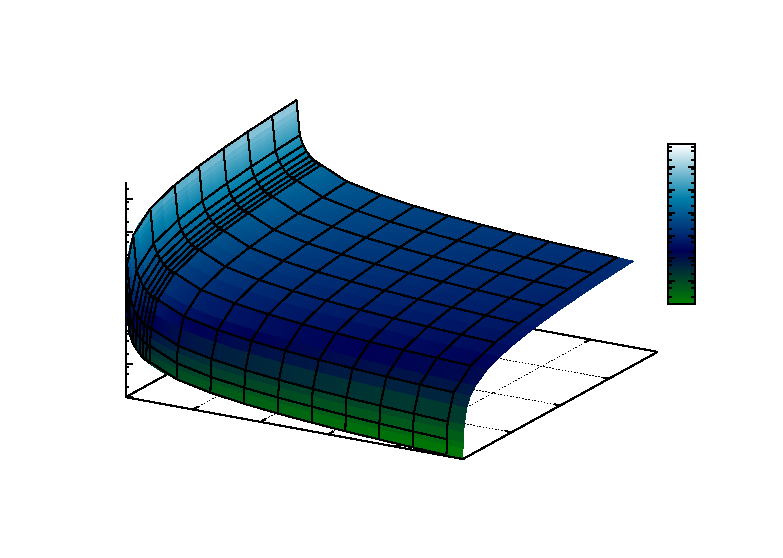
\includegraphics{ob-var-fig1}}%
    \gplfronttext
  \end{picture}%
\endgroup

%
%% Regular 2D plot
\begin{gnuplot}[terminal=epslatex,terminaloptions=color solid]
    set style data lines
    set key ins vert
    set log y
    set xlabel "Rounds"
    set ylabel 'Variance estimate $\sigma^2$' rotate
    set xtics 1,100,1000
    set xrange [1:1000]
    set yrange [*:1]
    plot 'est.txt' using ($4==1.0?$2:NaN):1 title '$\sigma_{ob}^2 = 1.0$' lt 1 lw 3, 'est.txt' using ($4==1.0e-3?$2:NaN):1 title '$\sigma_{ob}^2 = 0.0001$' lt 3 lw 3
\end{gnuplot}
\caption{Variance as a function of time (at $t = 0$, $\sigma$ is $50$)}
\label{fig:variance}
\end{figure}


\section{UCB1-Tuned}
In addition to local Thompson sampling, we implemented the UCB1 algorithm for 
comparing optimised Thompson samplers.

UCB1 \cite{Auer02UCB1} (Upper Confidence Bound) is a well-known algorithm for multi-armed bandits.
It is popular due to being very simple and reasonably performant. In comparison 
to LTS, it does not require any constant parameters, and in place of a given 
start estimate for the available arms the fist $K$ rounds are dedicated to 
initialising the arm estimates by playing every arm once.

UCB1-Tuned is a version of UCB1 that takes into consideration the estimate variance in addition to the estimate mean.
This should cause it to work better in practice.
In the remainder of this report, UCB1 means this improved algorithm.

The UCB1-Tuned strategy is simply to play the arm with index $i$ such that
\begin{displaymath}
    i = \operatorname*{argmax}_{j \in \{ 1..K \}} \left(\hat{\mu}_j + 
    \sqrt{\frac{\ln{n}}{n_j} \min(\frac{1}{4},\hat{V}_j)}\right)
\end{displaymath}
where 
\begin{displaymath}
    \hat{V}_j = \hat{\sigma}_j^2 + \sqrt{\frac{2\ln{n}}{n_j}}\text{.}
\end{displaymath}

$K$ is the number of available arms, $n_j$ the numer of times arm $j$ has 
been played, $n$ is the total number of plays, and $\hat{\mu}_j 
=\frac{(\text{cumulative reward for arm j})}{n_j}$.

In figure~\ref{fig:regretob} we compare the performance of LTS and UCB1.
We see that the optimal value for the \ob{} indeed causes LTS to perform better than UCB1.
The figure also illustrates why, when using LTS, it is important to make a good choice of observation noise.
In this case we see that the total regret achieved increases rapidly when the value is set too low, while it increases slightly as we move past the optimum.
With different setups we see similar results, although the slope after the optimum may be steeper or closer to zero.

\begin{figure}[htbp]
    \hspace*{-2.5cm}
    \begin{minipage}[c]{0.39\textwidth}
    \begin{gnuplot}[terminal=epslatex,terminaloptions=color solid]
    set style data lines
    set xlabel "Observation noise"
    set ylabel "Total regret"
    set xtics 0.048
    set mxtics 2
    #set arrow from 0.24,5 to 0.24,15 nohead lt 0
    plot [0.048:0.445] [5:15] '../data/cumulative/good-5.0,0.5_bad-4.0,0.5_est-0.0,50.0_num-4_obnoise-0.24_rounds-1000_reps-10000_algo-LTS_kind-Cumulative.data' using 3:(5000-$2) title "LTS" lw 3, (5000-4992.961761728431) title "UCB1" lc 3 lw 3
    \end{gnuplot}
    \end{minipage}
    \hspace*{7.5cm}
    \begin{minipage}[c]{0.49\textwidth}
    \banditsetup{5.0}{4.0}{0.5}{4}{1000}
    \end{minipage}
\caption{Resulting total regret from varying observation noise.}
\label{fig:regretob}
\end{figure}

% \section{Sample stuff}
% Some simple and useful latex formatting.
% 
% \subsection{Quotations and citing}
% It is explained in detail in \cite[Ch.20]{Norvig03} that
% 
% \begin{quotation}
% \noindent \textit{``the true hypothesis eventually dominates the Bayesian 
% predication. For any fixed prior that does not rule out the true hypothesis, the 
% posterior probability of any false hypothesis will eventually vanish, simply 
% because the probability of generating ``uncharacteristic'' data indefinitely is 
% vanishingly small.''}
% \end{quotation}
% 
% \subsection{Figures}
% This distribution, and its probability density function, is displayed in Figure 
% \ref{fig:gaussian_distr_pdf}.
% \begin{figure}[ht]
%     \center\includegraphics[width=10cm]{images/normal_distr_pdf}	
%     \label{fig:gaussian_distr_pdf}
%     \caption{The Normal distribution PDF.}
% \end{figure}
% 
% \subsection{Equations}
% By using these probabilities, and Bayes formula, we can derive the Bayes 
% classifier.
% \begin{equation}
%     P(\omega_i | \boldsymbol{x}, \mathcal{X}) = \frac{p(\boldsymbol{x}|\omega_i, 
%     \mathcal(X))P(\omega_i|\mathcal{X})}{\sum_{j=1}^{c}p(\boldsymbol{x}|\omega_j, 
%     \mathcal{X})P(\omega_j|\mathcal{X})},
%     \label{eq:bayes_formula_1}
% \end{equation}
% 
% when we can separate the training samples by class into $c$ subsets 
% $\mathcal{X}_1, \ldots, \mathcal{X}_c$, with the samples in $\mathcal{X}_i$ 
% belonging to $\omega_i$.
% 

            
    \chapter{Proposed Solution}
\label{ch:solution}
Approx. 10 pages

\section{Solution for single bandit}

We developed several ways to compute and visualise the needed data. A brute
force method calculating cumulative rewards for all given observation noises, a
method that, given the simulation parameters, employs a bandit approach to
calculating the best observation noise, and a method calculating instant
rewards at log-scale timesteps given the simulation parameters.

\subsection{Brute force solution}

By testing all the values in a given range it is possible to determine where the maximum lies.
Although this method is crude, it is helpful for gaining an indication towards what values are best or what values need more testing.
The downside of this solution is that many tests and much computation may be required, and most of the results generated are not interesting if we in reality are only looking for a (unique) maximum. 

\subsection{Bandit approach}

As the multi-armed bandit approach can be used to find the maximum of a
stochastic function, it fits perfectly to the task of finding the best
observation noise for a multi-armed bandit employing the local Thompson
sampling strategy.

\subsection{Measuring performance}

There are several ways to keep score and look at data from a bandit simulation.
First, one can look at the cumulative reward recieved by the player.
Second, there is the instant rewards, that is, the reward received by the player at a given time $t$.
By logging this one can easily see how the player increases its performance over time.
Third, a much used approach is to calculate regret.
In fact, the multi-armed bandit problem is often stated as a minimisation problem with respect to regret.
Last, the number of times the best arm is selected at any given time can be an interesting metric.


\section{Solution for Goore Game}




\section{Proposed solution / algorithm}

\subsection{The basic algorithm}

\subsection{Discussion of design issues}


\subsection{Algorithmic Enhancements}


\subsection{Discussion of the Parameter Space}


\section{Prototype}

\section{Justification of Claim to Originality}

\section{Valuation of Contribution}

\section{Alternatives}

    \newcommand{\exsetup}[6]{%
\begin{table}[htbp]
    \centering
    \begin{tabular}{lll}
        \toprule
        \multirow{2}{*}{Best arm}   & $\mu$    & #1 \\
                                    & $\sigma$ & #2 \\
        \multirow{2}{*}{Other arms} & $\mu$    & #3 \\
                                    & $\sigma$ & #4 \\
        \multicolumn{2}{l}{Number of arms}     & #5 \\
        \bottomrule
    \end{tabular}
    \caption{Simulation settings for figure~\ref{#6}}
\end{table}} 

\newcommand{\ob}{$\sigma_{ob}$}

\chapter{Results}
\label{ch:results}

Here we present a representative subset of the obtained results.
We provide graphs to visualise how different parameters influence the results.

Parameter values are likely to interact and impact the end result in different ways, and it may be difficult to capture these interactions directly.
By fixing all but one parameter and testing for a range of values for this parameter, we capture different aspects of how the optimal observation noise changes.

\section{Multiarmed Bandit}
Figure~\ref{fig:ex1} illustrates why, when using LTS, it is important to make a good choice of observation noise.
In this case we see that the total regret achieved increases rapidly when the value is set too low, while it increases slightly as we move past the optimum.
With different setups we see similar results, although the slope after the optimum may be steeper or closer to zero.
\begin{figure}[htbp]
    \begin{gnuplot}[terminal=epslatex,terminaloptions=color]
    set style data lines
    set grid
    set xlabel "Observation noise"
    set ylabel "Total regret"
    set key bottom
    plot "../data/bruteforce/good-5.0,2.0\_bad-4.0,4.0\_est-10.0,0.5\_num-2\_obstart-0.15\_obend-0.95\_obstep-0.01\_rounds-10000\_reps-10000.data" using 2:(column(1)==1000?(5000-column(3)):(1/0)) title ""
\end{gnuplot}
\caption{Resulting total regret from varying observation noise.}
\label{fig:ex1}
\end{figure}
\exsetup{5.0}{2.0}{4.0}{4.0}{2}{fig:ex1}

\begin{figure}[htbp]
    \begin{gnuplot}[terminal=epslatex,terminaloptions=color]
    set style data lines
    set grid
    set xlabel "Observation noise"
    set ylabel "Total regret"
    set log x
    set xrange [4:1000]
    plot "../data/instantrewards/good-5.0,2.0\_bad-4.0,4.0\_est-10.0,0.5\_num-2\_obnoise-0.51\_rounds-1000\_reps-100000\_algo-LTS.data" using 1:(5-column(2)) title "\\textsc{lts: 0.51}", "../data/instantrewards/good-5.0,2.0\_bad-4.0,4.0\_est-10.0,0.5\_num-2\_obnoise-0.6\_rounds-1000\_reps-100000\_algo-LTS.data" using 1:(5-column(2)) title "\\textsc{lts: 0.60}", "../data/instantrewards/good-5.0,2.0\_bad-4.0,4.0\_num-2\_rounds-1000\_reps-100000\_algo-UCB1.data" using 1:(5-column(2)) title "\\textsc{ucb1}"
\end{gnuplot}
\caption{Instant regret for UCB1 and LTS.}
\label{fig:ex2}
\end{figure}
\exsetup{5.0}{2.0}{4.0}{4.0}{2}{fig:ex2}

LTS is superior to UCB1, when the appropriate observation noise is selected.
In figure~\ref{fig:ex2} this superiority is clearly demonstrated:
Even though UCB1 performs quite good from the start it seems to stop reducing its regret after a while, whereas LTS converges towards zero regret.
The figure also illustrates how a suboptimal choice of \ob{} causes the algorithm to perform worse.

\begin{figure}[hbtp]
    \centering
    \begin{gnuplot}[terminal=epslatex,terminaloptions=color]
    set style data lines
    set grid
    set hidden3d
    set pm3d
    set xlabel "Arms" rotate
    set ylabel "Rounds" rotate
    set zlabel "Observation noise" rotate
    set log xy
    set xyplane 0
    set xtics 2
    set yrange [10:1000]
    set zrange [0.01:0.25]
    set palette rgbformulae 23,28,3
    splot "../data/bandit/good-5.0,0.5\_bad-4.0,0.5\_est-10.0,2.0\_num-2,5,10,50\_rounds-1000\_algo-UCB1.data" using 5:6:7 title ""
    \end{gnuplot}
\caption{Best observation noise varying with the number of arms. Values for when the number of arms is greater than rounds are not included.}
\label{fig:ex3}
\end{figure}
\exsetup{5.0}{0.5}{4.0}{0.5}{Variable}{fig:ex3}

We see generally that as the number of rounds increases, so does the optimal \ob{}.
This is especially apparent in figure~\ref{fig:ex3}, where we have varied the number of arms available to the player.
As the numer of possible actions increases, the optimal \ob{} decreases.
It makes intuitive sense because if there is a large number of arms then we need to be more greedy in our choice of arms, as most of the arms pulled for exploration’s sake will be suboptimal.

\begin{figure}[htbp]
    \centering
    \begin{gnuplot}[terminal=epslatex,terminaloptions=color]
    set style data lines
    set grid
    set hidden3d
    set pm3d
    set ylabel "Bad arm mean" rotate
    set xlabel "Rounds" rotate
    set zlabel "Observation noise" rotate
    set log x
    set xyplane 0
    set ytics 0.5
    set xrange [100:1000]
    set yrange [3:4.5]
    set view 40,36
    set palette rgbformulae 23,28,3
    splot "../data/bandit/good-5.0,0.5\_bad-(0.5,4.5,0.5),0.5\_est-10.0,2.0\_num-5\_rounds-1000\_algo-UCB1.data" using 6:3:7 title ""
    \end{gnuplot}
\caption{Best observation noise varying with the mean on the suboptimal arms. As the mean is lowered past 3 or so changing observation noise stops having an effect, so these numbers are excluded from this figure.}
\label{fig:ex4}
\end{figure}
\exsetup{5.0}{0.5}{Varying}{0.5}{5}{fig:ex4}
As the mean of the suboptimal arms get closer to $\mu^*$, more exploration can be afforded due to the small difference in payoffs.
This effect is illustrated in figure~\ref{fig:ex4}, where the optimal \ob{} increases along with the mean of the bad arms.

\begin{figure}[htbp]
    \begin{gnuplot}[terminal=epslatex,terminaloptions=color]
    set style data lines
    set grid
    set xlabel "Observation noise"
    set ylabel "Total regret"
    set yrange [13:15]
    set xrange [0.1:0.4]
    plot "../data/bruteforce/good-5.0,0.5\_bad-1.5,0.5\_est-10.0,2.0\_num-5\_obnoise-(0.01,0.4,0.01)\_rounds-1000\_reps-100000.data" using (column(1)==1000?column(2):1/0):(5000-column(3)) title ""
\end{gnuplot}
\caption{Sample from~\ref{fig:ex4}, with mean 1.5. This is the result of averaging over 100,000 runs.}
\label{fig:ex5}
\end{figure}
\exsetup{5.0}{0.5}{1.5}{0.5}{5}{fig:ex5}

In figure~\ref{fig:ex6} we see that changing the standard deviation of the suboptimal arms does not influence the best choice of observation noise, except for when the number of rounds is very low.
In fact, this seems to hold as long as the standard deviation is kept within reasonable limits.

\begin{figure}[hbtp]
    \centering
    \begin{gnuplot}[terminal=epslatex,terminaloptions=color]
    set style data lines
    set grid
    set hidden3d
    set pm3d
    set xlabel "[r]{\\shortstack{Bad arm \\\\ standard deviation}}"
    set ylabel "Rounds" rotate
    set zlabel "Observation noise" rotate
    set xyplane 0
    set xtics 0.5
    set ytics 200
    set cbtics 0.03
    set yrange [100:1000]
    set xrange [0:3.5]
    set zrange [0:0.6]
    set palette rgbformulae 23,28,3
    splot "../data/bandit/good-5.0,0.5\_bad-4.0,(0.1,3.5,0.2)\_est-10.0,2.0\_num-5\_rounds-1000\_algo-UCB1.data" using 4:(column(6)>99?column(6):1/0):7 title ""
    \end{gnuplot}
\caption{Varying standard deviation of the bad arms}
\label{fig:ex6}
\end{figure}
\exsetup{5.0}{0.5}{4.0}{Variable}{5}{fig:ex6}

\section{Goore Game}


    \chapter{Conclusion and further work}
\label{ch:conclusion}

\section{Conclusion}

By doing thousands of simulations we have discovered the observation noises that maximise LTS performance in a multitude of settings for the multi armed bandit.
We have also shown how the best observation noise varies with different parameters, thereby providing an improved intuition towards how the observation noise affects performance.

In the Goore game having more players only affects the optimal observation noise when you have a low white nose,
otherwise they all converge towards the same optimal observation noise. By changing the ratio, it effects the observation
noise in the way when it is closer to 0 or 1 in ratio the optimal observation noise is higher.
Observation noise also rises when the players have more time on their hands, since with more time each player may use more time 
to explore and find the best arm to pick and exploit. With higher white noise,the optimal observation noise do 
increase, and this do seam to be at a linear rate for each time step, with bigger variations at lower time steps.

\section{Contributions}
Our contributions consist mainly of an improved empirical and intuitive understanding of how the performance of the LTS strategy can be maximised by choosing correct observation noise.


\section{Further Work}
Use Gaussian processes to create models or graphs that can be used to inferr the optimal observation noise for a realistic subset of possible parameter configurations for the multi-armed bandit problem and the Goore game. Meaning that the Gaussian processes will use existing data to estimate unknown optimal observation noises. Currently all optimal observation noises are discovered through a brute-force approach thus if anyone requires a non-existent configuration of parameters it would be necessary to run the program with these new parameters. By employing Gaussian processes the user would be able to estimate the optimal observation noise by using existing data.



    \begin{singlespace}
        \bibliographystyle{IEEEtranS}
        % \bibliographystyle{plain}
        % \bibliographystyle{apalike}
        \bibliography{bib/web}
    \end{singlespace}

    \printglossary

\end{document}

